\section{Manuel d'utilisation}

Cette application débute avec une boîte de dialogue qui laisse le choix entre deux rôles : Maître de Jeu (MJ) ou Joueur. Si "MJ" est choisi, l'application se lance en tant que serveur pour accueillir les joueurs. Si "Joueur" est choisi, un assistant ce connexion apparaît pour choisir à quel serveur se connecter. Dans les deux cas, un pseudonyme est demandé; si le champs n'est pas rempli la personne se nommera "guest" \\

L'interface qui se présente comporte un Chat, un gestionnaire de tours et le lanceur de dés. Le Chat contient la liste des utilisateurs et permet aux joueurs et au MJ de communiquer. De plus, le chat possède des commandes qui s'introduisent par un /. Les commandes implémentées sont :

\begin{description}
	\item[/help] \hfill \\
		Affiche l'ensemble des autres commandes disponibles du chat avec les indications d'utilisation.
	\item[/nickname <pseudo>] \hfill \\
		Modifie le pseudo par celui qui suit la commande.
	\item[/roll <nombre de dés>d<valeur max du dé>] \hfill \\
		Roule un nombre de fois voulu du dé choisi. Peut s'utiliser en chuchotement. Peut lancer de multiples dés en les séparant par un '+' ou un '-'. Peut ajouter une valeur fixe au résultat final en ne précisant pas la partie "d<valeur max du dé>.
	\item[/whisper <utilisateur> <message>] \hfill \\
		Envoie un message privé au joueur indiqué. Peut cibler des utilisateurs multiples en les séparant par '|'.
\end{description}

\begin{figure}[h!]
	\centering
	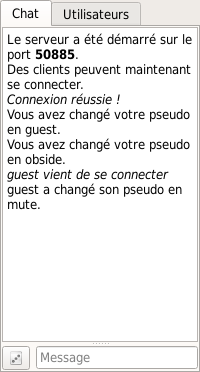
\includegraphics[scale=0.5]{img/chat_mj.png}
	\hspace{10 mm}
	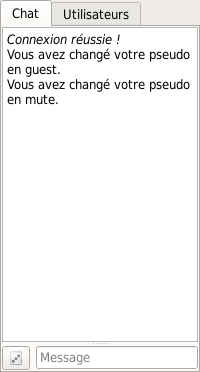
\includegraphics[scale=0.5]{img/chat_player.png}
	\caption{Chat MJ (à gauche) et chat Joueur (à droite)}
\end{figure}

Le Chat propose également une liste d'utilisateurs connectés. Un clic droit sur un ou plusieurs utilisateurs de cette liste affiche un menu contextuel donnant accès à des actions : Envoyer un message, et Lancer les dés.
La première action prépare un message privé à un ou plusieurs utilisateurs, la seconde lance les dés sélectionnés dans le lanceur de dés et envoie le résultat uniquement aux utilisateurs sélectionnés.


\begin{figure}[h!]
	\centering
	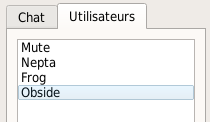
\includegraphics[scale=0.5]{img/chat_userlist_1.png}
	\hspace{10 mm}
	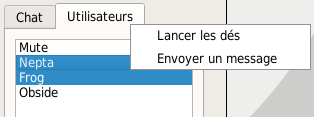
\includegraphics[scale=0.5]{img/chat_userlist_2.png}
	\caption{Liste d'utilisateurs (à gauche) et menu contextuel proposant des actions sur les utilisateurs sélectionnés (à droite)}
\end{figure}

\newpage

Le lanceur de dés propose les dés les plus utilisés et permet de choisir pour chaque type de dé, le nombre de fois que celui-ci doit être lancé. Initialement, les compteurs sont à zéro. Pour augmenter le nombre dés à lancer, il faut clicker gauche sur le bouton correspondant ou utiliser la molette de la souris pour faire varier le nombre en étant sur le bouton. De même, pour décrémenter les dés il suffit de clicker droit ou de scroll vers le bas sur un bouton. On peut ensuite décider de lancer les dés sur le chat (lancé public) ou de lancer les dés en privé (lancé caché). Un lancé privé n'est visible que par celui qui l'effectue, et est principalement utilisé par le MJ. Il est possible de réinitialiser tous les compteurs.

\begin{figure}[h!]
	\centering
	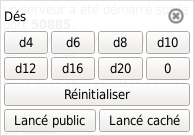
\includegraphics[scale=0.5]{img/dice_manager.png}
	\caption{Lanceur de dés}
\end{figure}

Le gestionnaire de tours est un outil qui permet au MJ de gérer ses combats. Les icônes sur la droite du gestionnaire permettent d'ajouter et de retirer des tours à la liste (voir figure \ref{fig:turnManager}). Ceux-ci peuvent par exemple représenter les tours des personnages joueurs, non joueurs et/ou des lancers de sorts. Le MJ peut également réordonner les tours à l'aide du glisser-déposer. Toutes les actions effectuables à la souris disposent également d'un équivalent en raccourcis clavier, il est par exemple possible de naviguer entre les tours et de les réarranger à l'aide des flèches du clavier. Pour sélectionner plusieurs éléments à l'aide du clavier, il suffit de maintenir la touche Maj enfoncée et d'apuyer sur les flêches. Pour en déplacer, il suffit d'en sélectionner puis de mainternir Ctrl enfoncée et d'appuyer sur les flêches. Enfin, lorsque des utilisateurs se connectent ils sont automatiquement ajoutés dans le gestionnaire de tour.

\begin{figure}[h!]
	\centering
	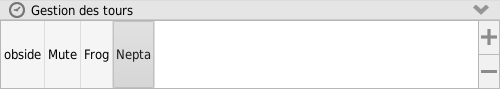
\includegraphics[width=0.7\textwidth]{img/turn_manager.png}
	\caption{Gestionnaire de tour}
	\label{fig:turnManager}
\end{figure}